\chapter{Results}
\label{results}

\minitoc

In this chapter relevant articles gathered on ...

\newpage

\section{Introduction and Clarification}

\begin{table}[H]
\begin{center}
    \begin{tabular}{| p{5cm} | p{3.7cm} | p{1cm} | p{4cm} |}
    \hline
    \textbf{Article Name} & \textbf{Author(s)} & \textbf{Year} & \textbf{Keywords} \\ \hline
    Inter-team Coordination in Large-scale Globally Distributed Scrum: Do Scrum-of-Scrums Really Work? & Maria Paasivaara, Casper Lassenius, Ville T. Heikkilä & 2012 & Agile Software Development; Distributed Scrum; Global Software Engineering; Inter-team Coordination \\ \hline
    Communities of Practice in a Large Distributed Agile Software Development Organization – Case Ericsson & Maria Paasivaara, Casper Lassenius & 2014 & Communities of Practice; Large-scale Agile Software Development; Scaling Agile \\ \hline
    Operational Release Planning in Large-scale Scrum with Multiple Stakeholders – A Longitudinal Case Study at F-Secure Corporation & Ville T. Heikkilä, Maria Paasivaara, Kristian Rautiainen, Casper Lassenius, Towo Toivola, Janne Järvinen & 2015 & Agile Software Development; Scrum; Large Projects; Release Planning; Software Project Management \\ \hline
Towards a Governance Framework for Chains of Scrum Teams & Jan Vlietland, Hans van Vliet & 2015 & Agile; Chain of Scrum Teams; Coordination; Priority; Alignment; Predictability \\ \hline
    \end{tabular}
    \caption{Summary of articles used in this chapter.}
    \label{soauitc}
\end{center}
\end{table}

\begin{table}[H]
\begin{center}
    \begin{tabular}{| p{4cm} | p{8cm} |}
    \hline
    \textbf{Role} & \textbf{Description of role} \\ \hline
    Scrum master & \\ \hline
    Functional architect & \\ \hline
    Technical architect & \\ \hline
    Tester & \\ \hline
    Developer & \\ \hline
    \end{tabular}
    \caption{Team roles present in Scrum teams.}
    \label{trpist}
\end{center}
\end{table}

\begin{figure}[H]
\centering
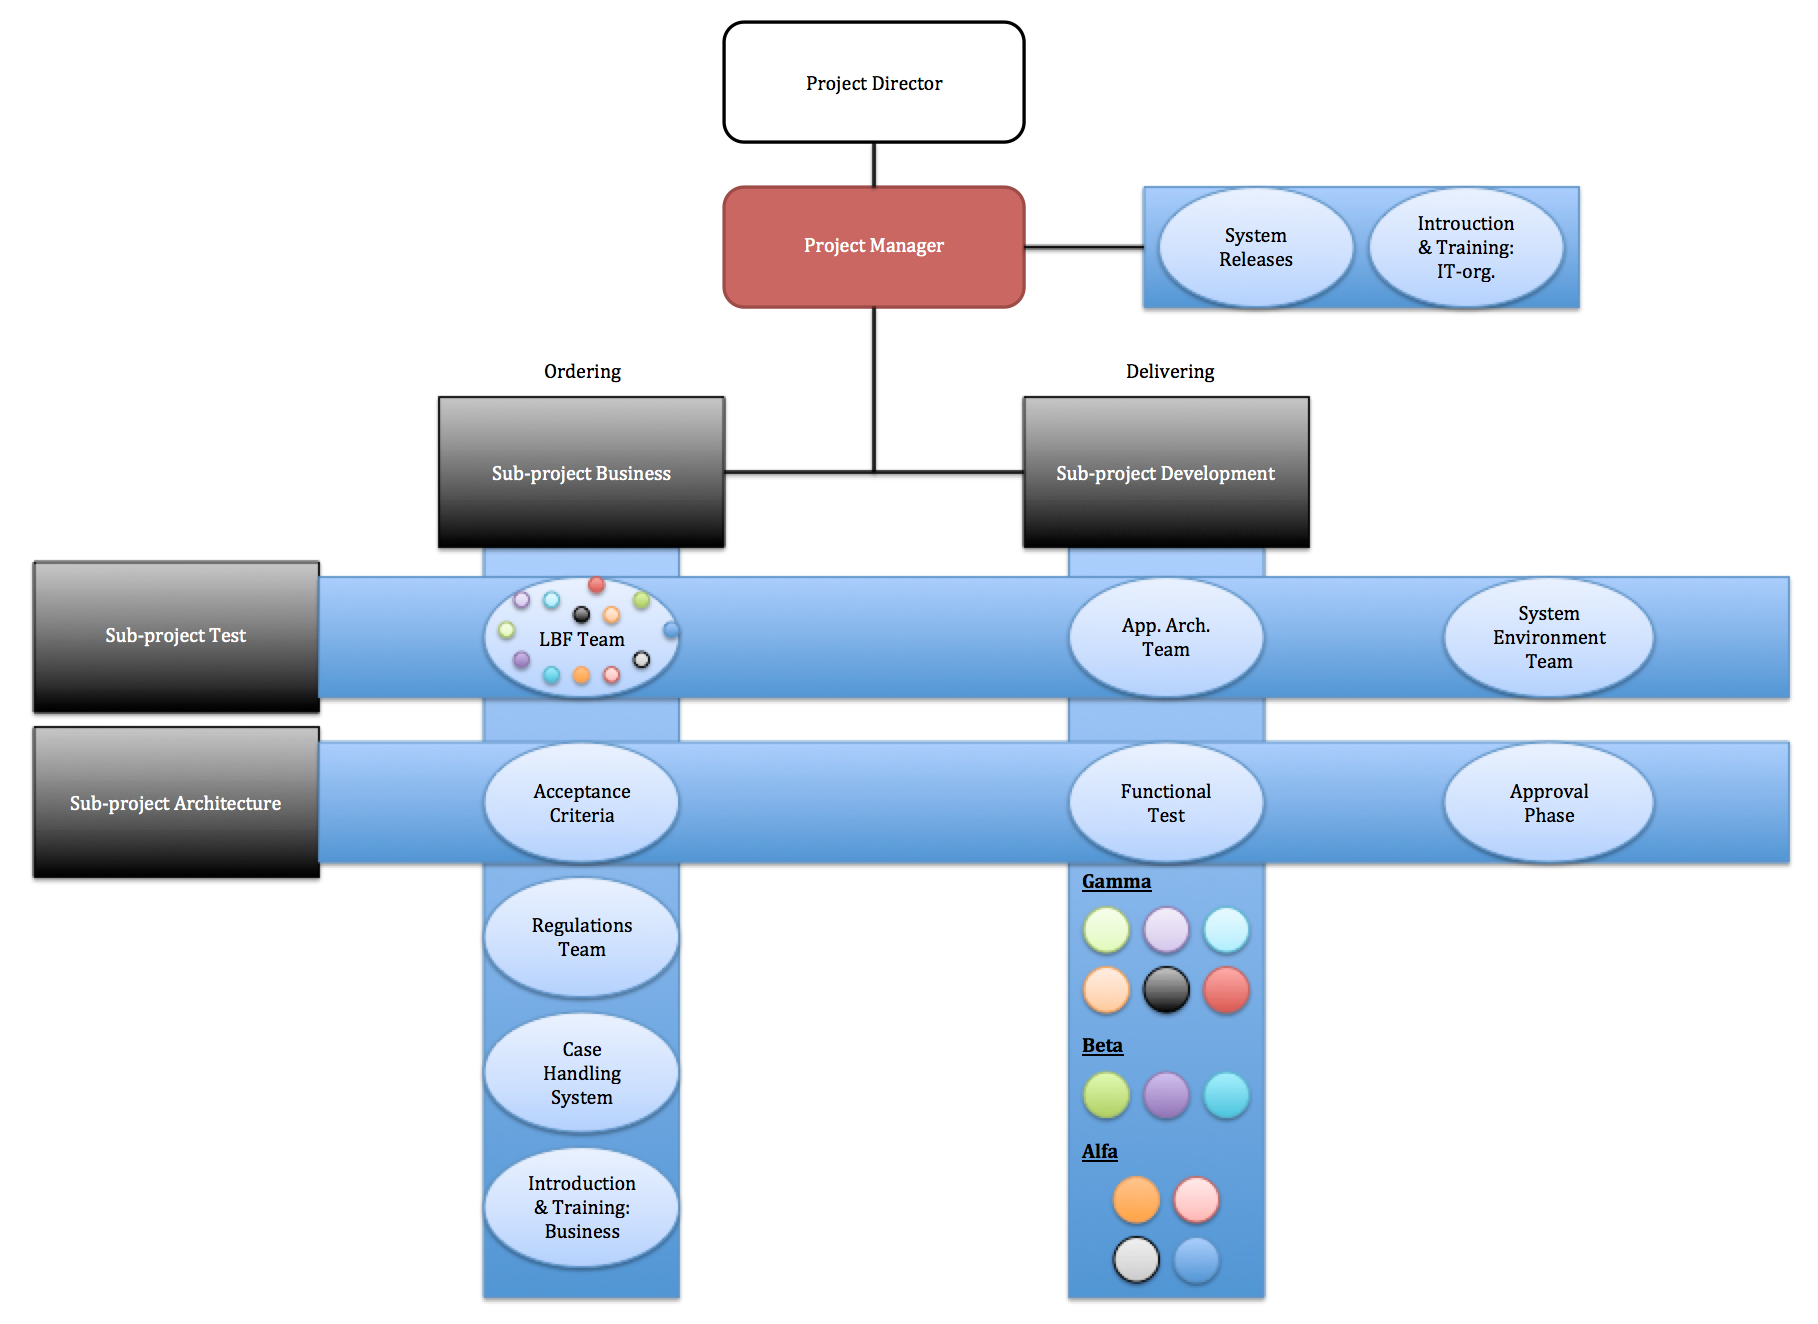
\includegraphics[trim = 40mm 0mm 7mm 0mm,width=180mm]{images/omega_organisation.png}
\caption{Omega-project's organisation.}
\label{omega}
\end{figure}

\begin{figure}[H]
\centering
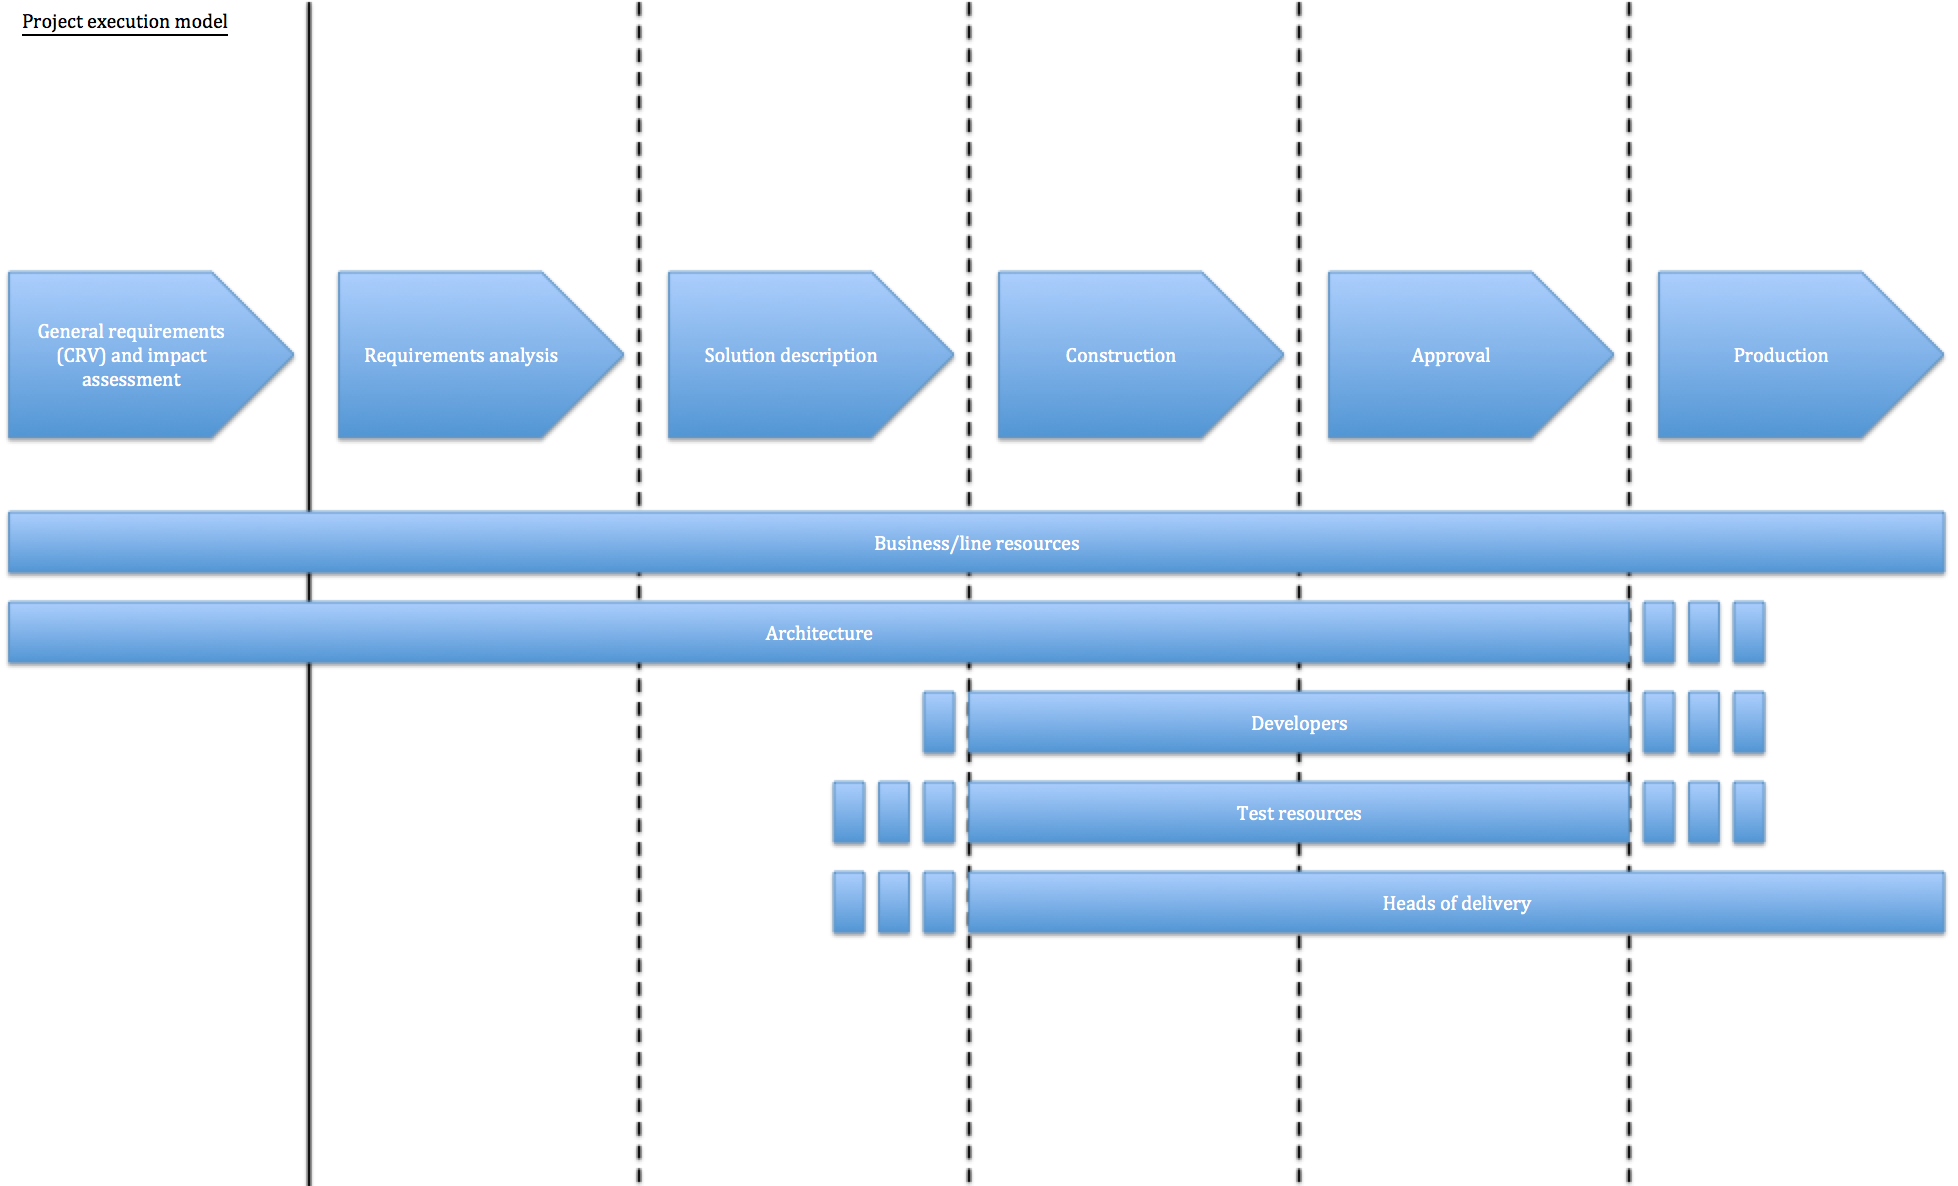
\includegraphics[angle=90, trim = 0mm 0mm 20mm 0mm,width=160mm, height=230mm]{images/execution_model.png}
\caption{Project execution model.}
\label{project_execution}
\end{figure}

\begin{figure}[H]
\centering
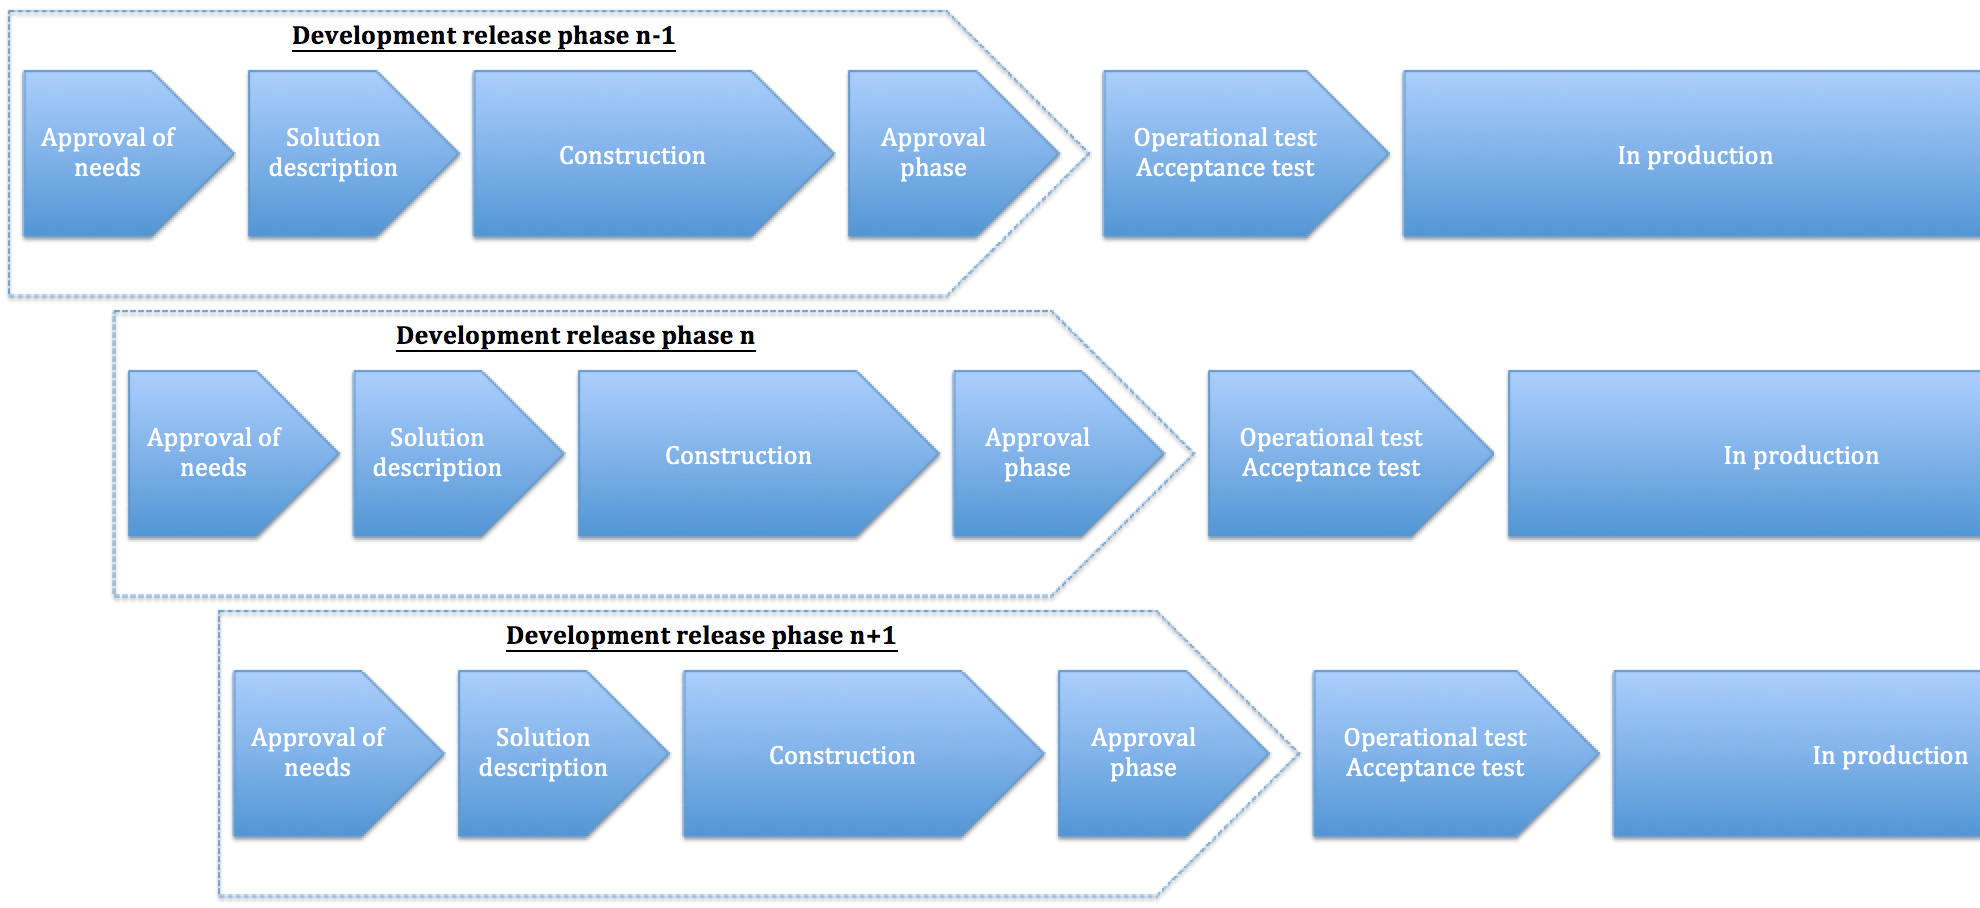
\includegraphics[angle=90, trim = 0mm 0mm 20mm 0mm,width=160mm, height=230mm]{images/initial_development_process}
\caption{Initial development process.}
\label{initial_development_process}
\end{figure}

\begin{table}[H]
\begin{center}
    \begin{tabular}{| p{6cm} | p{9cm} |}
    \hline
    \textbf{Coordination mechanism} & \textbf{Description of mechanism} \\ \hline
    Metascrum & A meeting similar to Scrum of Scrums but with less details which was held twice per week. Attending the metascrum was the project leaders and all the sub-project leaders from test, architecture, business and development. A ``technical metascrum'' was tried, but was shortly shut down after initiation. \\ \hline
    Planning day & Ulike nivåer (prosjekt, leverandør og team), utviklerforum (leverandørnivå, ikke på tvers av hele prosjektet), Iterasjonsoppstart(?) \\ \hline
    Dependency meeting & A meeting held between all Scrum masters from the Alpha, Beta and Gamma teams. This meeting was held on the ``Planning day'' where the focus was on discovering dependencies across Scrum teams. However, these meetings faded away early on because of the dependencies being discovered and handled elsewhere. \\ \hline
    Solution description / ``Master plan'' & negotiation and estimation meetings part of solution description meetings \\ \hline
    Wiki/Jira/Confluence & \\ \hline
    Jabber & Jabber was introduced as an instant messaging service in the Omega-project after being identified as something needed in one of the Open-space sessions. Project members could ask both formal questions, e.g., technical questions, and informal questions or activities, e.g., wine lotteries. \\ \hline
    Open-space & An arena held on a voluntary and need basis, which was used for exchanging experiences. Only used during a few of the releases. Participants suggested the topics beforehand, leading to agendas for open-space sessions. \\ \hline
    Lunch seminars & Kind of similar to the ``open-space'' sessions. Typically two to three topics were held by project-personnel on relevant and interesting topics, often regarding themes correlated to the current situation of the project. As with the ``open-space'' session these seminars were also held on a certain period of the project before fading away. \\ \hline
    Demo &  \\ \hline
    Front-end meeting & The front-end developers worked with a complex framework called Flex. Because of this a lot of coordination had to be handled between teams working with this framework from all organisations. Therefore, front-end meetings where held were typically the most prominent Flex-developers were present. \\ \hline
    Technical architecture forum &  \\ \hline
    Architecture board & \\ \hline
    Business & \\ \hline
    Bug-board meetings  & \\ \hline
    \end{tabular}
    \caption{Coordination mechanisms used across the whole Omega-project.}
    \label{cmuatwo}
\end{center}
\end{table}

%Feil å kalle det sub-projects?
\begin{table}[H]
\begin{center}
    \begin{tabular}{| p{6cm} | p{9cm} |}
    \hline
    \textbf{Coordination mechanism} & \textbf{Description of mechanism} \\ \hline
    Scrum of Scrums (SoS) & Scrum of Scrums were meetings held by all organisations (Alpha, Beta and Gamma) ranging from two to three times per week. In these meetings all Scrum masters from the corresponding organisation, as well as project management (project leader, test leader, head technical architect, head functional architect, business leader and development leader). The main goal of the SoSs was to identify and handle obstacles. There were also held a few SoS meetings across organisations to handle potential changes to the contracts. \\ \hline
    Stand-up &  \\ \hline
    Pre-planning day & \\ \hline
    Technical corner & The ``technical corner'' was a meeting Beta had in an early stage of the project. It was held on Fridays for about 1-1,5 hour. Here team architects presented important themes for the Beta-members. After a while it was shut down because of lack of interest and topics. \\ \hline
    Experience forum & The experience forum was an arena established in the Alpha-organisation for exchanging experiences. Here Scrum masters and the development manager met to discuss topics such as retrospectives, the planning day, and how work was performed by the Alpha-organisation's Scrum teams. It could be seen as a coaching-session with exchange of ideas and thoughts. \\ \hline
    Board discussion & \\ \hline
    Retrospective & Different levels at Alpha (team, solution description and project management), Global retrospektiv testet ut på Beta \\ \hline
    Technical architecture meeting & \\ \hline
    Functional architecture meeting & \\ \hline
    Supplier meeting & Alpha \\ \hline
    Meeting about queue & Alpha \\ \hline
    \end{tabular}
    \caption{Coordination mechanisms used across sub-projects in the Omega-project.}
    \label{cmuasito}
\end{center}
\end{table}

\begin{table}[H]
\begin{center}
    \begin{tabular}{| p{6cm} | p{9cm} |}
    \hline
    \textbf{Mechanism/Aspect} & \textbf{Description} \\ \hline
    Co-location & \\ \hline
    Informal communication & \\ \hline
    Trust & \\ \hline
    Joint coffee break & Alpha (generelt?) \\ \hline
    Pair-programming & \\ \hline
    Self-organising & \\ \hline
    Rotation of team members & \\ \hline
    Rotation of team placement & \\ \hline
    Alfa/Beta-personnel placed in Gamma teams & \\ \hline
    Project management in same location & ``Walking around, talking around'' \\ \hline
    Continuous planning & \\ \hline
    3-level hierarchy from product owner & \\ \hline
    \end{tabular}
    \caption{Other coordination mechanisms and important aspects.}
    \label{ocmaia}
\end{center}
\end{table}